\section{Global class diagrams}
The following schemas (\ref{fig: Class diagram of the platform}, \ref{fig: Class diagram of the XML management} and \ref{fig: Class diagram with the links between the platform and the XML part})  are class diagrams that describe the global architecture of the \ac{siconos} platform.
	\begin{figure}
	\begin{center}
	\includegraphics[scale=1.2, clip]{figure/kernel2.eps}
	\caption{Class diagram of the platform}
	\label{fig: Class diagram of the platform}
	\end{center}
	\end{figure}
	
	\begin{figure}
	\begin{center}
	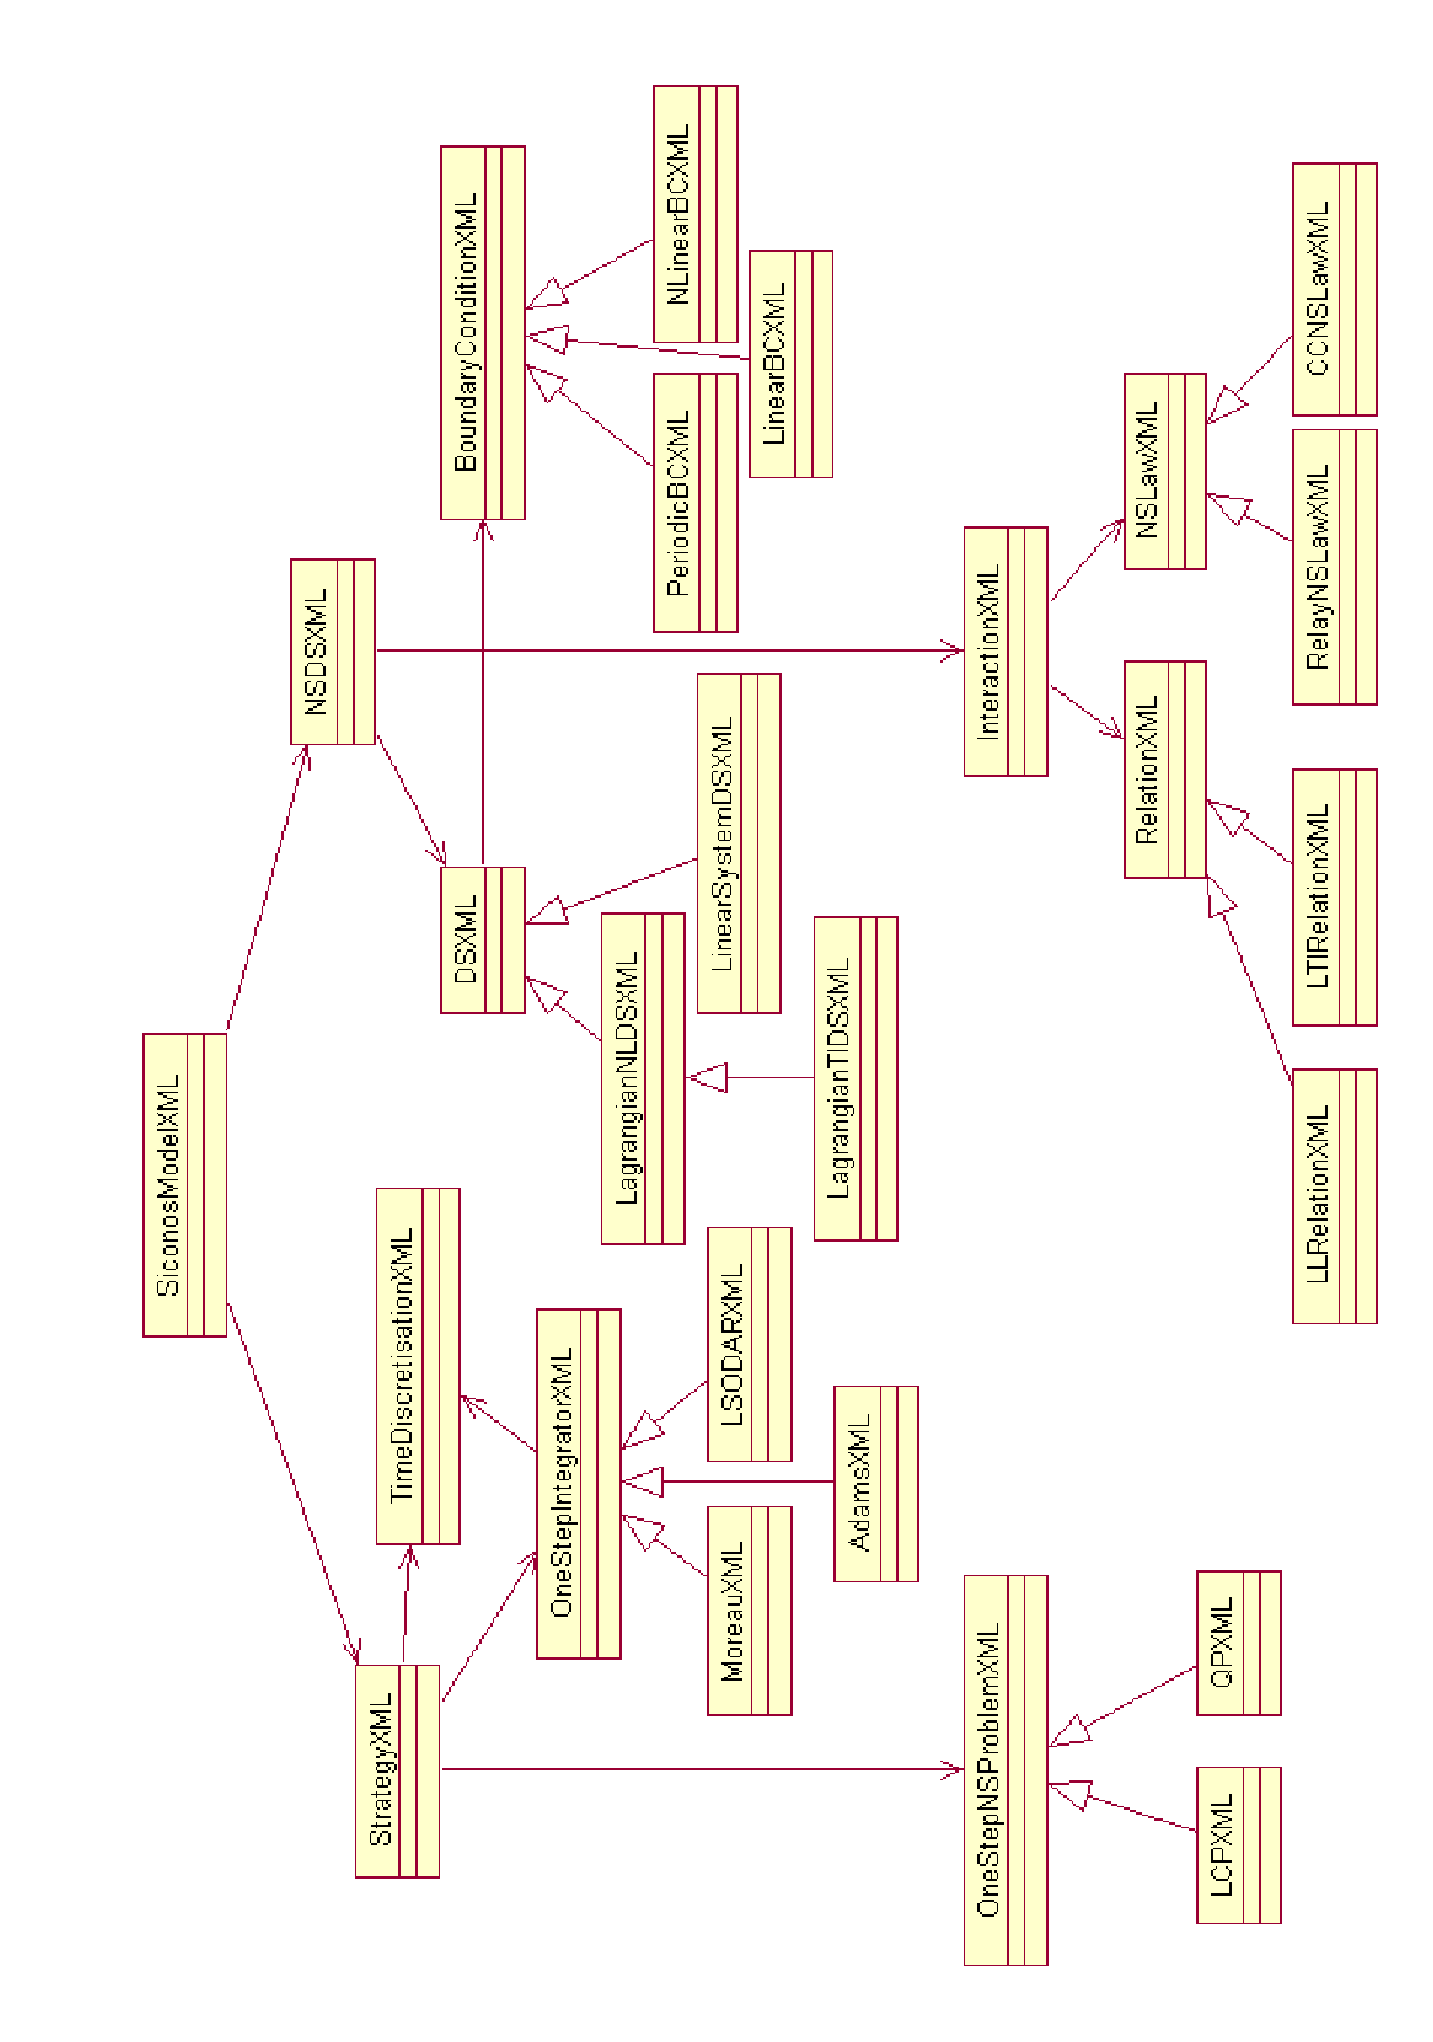
\includegraphics[scale=0.75, clip]{figure/schemaXML.eps}
	\caption{Class diagram of the XML management}
	\label{fig: Class diagram of the XML management}
	\end{center}
	\end{figure}
	
	\begin{figure}
	\begin{center}
	\includegraphics[scale=1.2, clip]{figure/platform.eps}
	\caption{Class diagram with the links between the platform and the XML part}
	\label{fig: Class diagram with the links between the platform and the XML part}
	\end{center}
	\end{figure}


\section{Detailed Design}
\subsection{Code documentation}
\cf~Siconos source code documentation generated by Doxygen

\subsection{Modeling tools update}
The \ref{fig: Class diagram of DSInputOutput and EqualityConstraint added} class diagram represents the EqualityConstraint and DSInputOutput classes (and inherited classes).
	\begin{figure}
	\begin{center}
	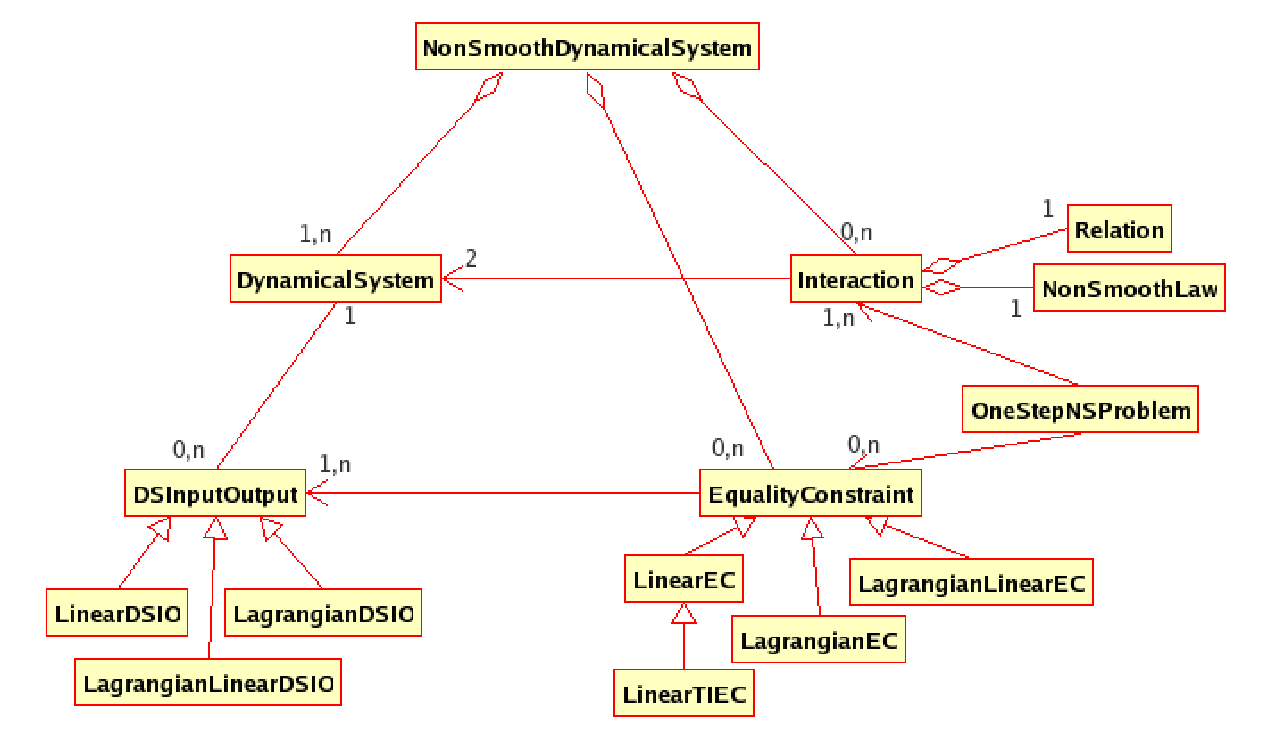
\includegraphics[scale=0.85, clip]{figure/EC.eps}
	\caption{Class diagram of DSInputOutput and EqualityConstraint added}
	\label{fig: Class diagram of DSInputOutput and EqualityConstraint added}
	\end{center}
	\end{figure}
	
\subsubsection{DSInputOutput classes}

\subsubsection{EqualityConstraint classes}



\pagebreak

\section{SiconosMemory}
	
This section explains the global functionning of the class SiconosMemory. This class aims to store some SiconosVectors of previous steps of the simulation.\\
For example, in a Dynamical System, we can save the state of the system. This mechanism is needeed by certain integrators. \\

The attributes of the class are :
\begin{itemize}
\item The maximum number the memory can store.
\item The current number of SiconosVectors stored in the Memory
\item A \acs{stl} vector of pointers on SiconosVector.
\item A pointer on SiconosMemoryXML, used if the memory must be saved in a \ac{xml} file.
\end{itemize} 

The class SiconosMemory is designed to avoid useless copies of SiconosVectors. For the storage of a SiconosVector, there is only one copy : when it enters in the SiconosMemory. Next, the moves of position in the Memory are only done with adresses of pointers. \\
 
We have designed the SiconosMemory to be used preferably with a constant maximum size. In fact, the size is generally known before the initialization of the memory, because each kind of integrator needs a constant number of values of previous steps of the simulation to integrate a system. \\

The management of the relation between SiconosMemory and the \ac{xml} file is the classical one used in the plateform. There are two functions in the SiconosMemory to load or save it in the \ac{xml} DOM tree. The object SiconosMemoryXML realizes this transfer of data.
We chose this method, with a specified \ac{xml} object instead of saving directly the memory with functions in SiconosDOMTreeTools in order to respect the philosophy defined in the global architecture. Only the basic objects of the platform, like numbers, vectors and matrices have not a xml manager. %In fact, if we had chosen to load and save directly the SiconosMemory in the DOM tree, why could we not do the same with eveything ? \\

\begin{figure}[h]
\begin{center}
\includegraphics[scale=0.75, angle=-90, bb=20 40 330 710, clip]{figure/SiconosMemory.ps}
\caption{class diagram of SiconosMemory}
\label{fig: class diagram of SiconosMemory}
\end{center}
\end{figure}

\pagebreak
\section{SiconosVector}

After the first version of the platform, it appeared that the class SiconosVector was not satisfactory. A new version is now implemented with a different approach. An abstract interface represents now the vector and functionnalities it can assume (see \ref{fig: class diagram of SiconosVector}). \\

The class SimpleVector represents basic double vector and is totally in accordance with the interface. Its core is a Lapack double vector (class LaVectorDouble). \\

The class CompositeVector represents compound vectors and is partially in accordance with the interface. Its functionnalities are limited because this class do not contain any data. It only point on other vectors, so certain operations could have hazardous border-effects. In a general way, we recommand to use this vector in :

\begin{itemize}
	\item	left member of affectation (CompositeVector = ...).\\
	
	\item	most-right-possible in operators +, -, /, * with other vectors (the vector is then in strictly read-only mode : Vector = 		... + vector + CompositeVector).
\end{itemize}

\textit{Remember, when a CompositeVector is affected or change by an operation, the vectors it references too.} \\

\begin{figure}[h]
\begin{center}
\includegraphics[scale=0.75, bb=20 570 530 830, clip]{figure/SiconosVector.ps}
\caption{class diagram of SiconosVector}
\label{fig: class diagram of SiconosVector}
\end{center}
\end{figure}
